\documentclass[10pt]{IEEEtran}

\usepackage{blindtext}
\usepackage{titling}
\usepackage[style=ieee]{biblatex}
\usepackage{indentfirst}
\usepackage{algorithm}
\usepackage{algpseudocode}
\usepackage{float}
\usepackage{caption}
\usepackage{subcaption}
\usepackage{graphicx}
\usepackage{cleveref}

\bibliography{sources.bib}

\setlength{\columnsep}{1cm}

\title{Rendering Photorealistic Computer Graphics Using Ray-Tracing}
\author{Zach Clayburn}

\pretitle{
    \begin{center}
        \Huge\bfseries
}
\posttitle{
    \end{center}
}

\renewenvironment{abstract}{
    \small
    \begin{center}
    \bfseries \abstractname\vspace{-.5em}\vspace{0pt}
    \end{center}
    \list{}{%
        \setlength{\leftmargin}{4mm}
        \setlength{\rightmargin}{\leftmargin}
    }
    \item\relax
}{\endlist}

\begin{document}

\maketitle

% \begin{multicols*}{2}

\begin{abstract}

Modern computer generated imagery is predominantly done using a family of algorithms called
ray-tracing. These unlike traditional rasterization rendering, these algorithms simulate rays of
light as they travel around a scene and are captured by a virtual camera. A basic backward
ray-tracing renderer is implemented, its runtime complexity is discussed, and its output is
demonstrated.

\end{abstract}

\section*{Introduction}

In the past few decades that they have existed, computer graphics have evolved and improved far
beyond what was initially possible. Where it once was an accomplishment to create a simplistic image
that roughly approximated the real world, computers can now create imagery that is near
indistinguishable from reality. Improvements in both the algorithms used and the hardware running
those algorithms have made these improvements possible. A key example of one of these improvements
is the introduction of ray-tracing algorithms.

Early computer graphics would use a process called rasterization, where the color of each pixel is
determined by computing the color of the object in front of each pixel, and then adding more effects
through post-processing steps called shading. This method can be quite effective and much effort has
been put into optimizing and improving this technique. Ray-tracing, however, takes a fundamentally
different approach, and actually simulates individual rays of light as they travel through the scene
being rendered, resulting in images that are much closer to real photography. While this technique
can be conceptually simple to understand and implement, it is extremely computationally expensive.

\section*{Motivation}

This paper discusses the basics of ray-tracing, and goes over my implementation of a simple ray
tracing renderer. I selected this topic because I have always been interested in computer graphics.
From video games to animated films, the topic has always been fascinating to me. In the past, I have
experimented with traditional raster based rendering libraries (OpenGL, Vulkan), and I have a fairly
decent working knowledge of how those processes work. I have not, however, dealt with any
ray-tracing based rendering, and wanted to learn more about how it works. I had heard of an
excellent book available online that walks through the process of writing a ray-tracing rendering
engine \cite{Shirley2020RTW1}, and given the opportunity to complete this assignment, I decided this
would be a great algorithm to study.

\section*{Background}

As mentioned previous, 3D computer graphics used to be created using rasterization and shading. This
process involves computing each pixel color in several shading passes, adding more detail with each
pass. The base pass determines the base color of each pixel, and then effects like lighting, motion
blur, are added with each subsequent pass. The advantage of this style of rendering is that it can
be done incredibly fast, with highly efficient algorithms and purpose built hardware able to
massively parallelize the process. Because of this speed, this technique is still used in real-time
applications (e.g. video games), where images must be produced at a minimum rate of thirty every
second.

When the render time is not an issue, ray-tracing is a much more desirable choice. Because the
process involves simulating light similar to how it behaves in the real world, the quality of the
images is much higher. Most computer generated imagery used in movies, like special effects and
fully animated movies, are rendered with a ray-tracing based renderer.

While up to this point I have been talking about ray-tracing as if it was a singular technique, it
really describes a category of similar algorithms. To illustrate, I will give a (non-exhaustive)
list of varieties of ray tracing \cite{stanfordRayTracingTypes}:
\begin{itemize}
    \item \textbf{Forward:} In this method, light rays are simulated emitting from a light source,
    and a virtual camera records when those light rays collide with it, and the image is generated
    from those collisions. This method is the most accurate, as it is a direct simulation of
    reality. A major drawback of this method is that many computations go to waste, as not all rays
    emitted actually end up contributing to the image.
    \item \textbf{Backward:} In this method, rays are simulated backwards in time. Rays are computed
    at the virtual camera corresponding to each pixel, and case outward to find what object is
    visible, in a method similar to rasterization. The difference is that, after colliding with the
    principal object is hit by the ray, it is simulated bouncing around, just as a real photon
    would, until it meets a light source. While this is more efficient, in some cases it is less
    accurate than the forward method.
    \item \textbf{Hybrid:} Hybrid methods are an attempt to compromise speed and accuracy, and
    involve performing some forward ray-tracing on a scene, and then stores that data. It then
    performs backward tracing, and uses the stored data from the forward step to compute the color.
\end{itemize}

\section*{Implementation}

\begin{algorithm}[b]
    \caption{Backward Ray Tracing Algorithm}\label{alg:render}
    \scriptsize
    \begin{algorithmic}[1]
        \Procedure{Render}{$imageWidth, imageHeight,$\par
            \hskip\algorithmicindent $scene, samplesPerPixel, maxRecursion$}

        \State $camera$$ \gets \textsc{getCamera}(imageWidth, $\par
            \hskip\algorithmicindent$imageHeight, scene)$

        \State $image \gets \textsc{createImage}(imageWidth, $\par
            \hskip\algorithmicindent$imageHeight)$

        \For {$x\gets 0\ldots imageWidth$}
            \For {$y\gets 0\ldots imageHeight$}
                \State $color \gets (0,0,0)$
                \For{$0\ldots samplesPerPixel$}
                    \State $u \gets (x + \textsc{Random}(-0.5,0.5))$
                    \State $v \gets (y + \textsc{Random}(-0.5,0.5))$
                    \State $ray \gets camera.\textsc{getRay}(u,v)$
                    \State $color \gets color + $\par
                        \hskip\algorithmicindent$\textsc{rayColor}(ray, scene, maxRecursion)$
                \EndFor
                \State $image.\textsc{at}(x, y)$\par
                \hskip\algorithmicindent$ \gets color / samplesPerPixel$
            \EndFor
        \EndFor

        \EndProcedure
    \end{algorithmic}
\end{algorithm}

For my implementation, I went with a backward ray tracing algorithm. As can be seen in
\cref{alg:render}, the actual render loop is not overly complicated. The image is iterated over
pixel by pixel, and a set number of samples are taken for each pixel. To take a sample, a random
number is added to the x and y components, which are then normalized by the image dimensions. The
reason multiple samples are taken for each pixel is to provide anti-aliasing, so that the pixels on
the edge of a shape will not abruptly transition from one color to another, but blend smoothly
between to two colors. Additionally, because some of the ray computations are stochastic in nature,
these multiple samples help to reduce noise by decreasing the visual weight of outliers of those
stochastic processes.

The process for computing the actual color, what takes place in the \textsc{GetColor} function in
\cref{alg:getcolor}, is where the similarity to rasterization ends. The ray is checked against all
the objects in the scene, to see if it impacted any of them. If no objects are struck, then it is
assumed that the ray that came from that direction is from the global light source (e.g. the sun),
and so it is colored according to whatever global illumination is set up for the scene. If an object
or objects are impacted then the nearest object is found. Then the material is used to "scatter" the
ray. What the process of scattering is depends on the material. Then, the function is recursively
called with that scattered ray to determine where that ray would have come from and what color it
would be. Because this is a recursive function, there is the possibility of a ray getting trapped
and taking an indeterminately long time to reach a light source. To prevent wasting time on a ray
that has no chance of contributing significantly to the image, or even to get stuck in an infinite
recursion, the depth parameter is used to limit how deep the recursion will go, and just returns
black if that limit is reached.

As for materials, my implementation has two kinds: lambertian and metal. Lamberitan materials have a
diffuse surface, meaning they scatter the light in a random direction from the point of impact while
removing a portion of the energy from that light, which leads to a flat looking surface. The other
material, metal, reflects light beams in a deterministic method, resulting in reflections showing up
in the surface of the object. Metal materials also have another property, roughness, that adds a
small amount of randomness to the reflection, which results in a surface looking rough, and similar
to a lambertian material. This property varies from 0 (completely smooth), to 1 (completely rough).

\begin{algorithm}[b]
    \caption{Procedure for Computing ray color}\label{alg:getcolor}
    \scriptsize
    \begin{algorithmic}
        \Procedure{getColor}{$ray, scene, depth$}
        \If{$depth = 0$}
            \State \Return $(0,0,0)$
        \EndIf
        \State $hitRecord \gets scene.\textsc{computeHit}(ray)$
        \If{$hitRecord.hit$}
            \State $object\gets hitRecord.nearest$
            \State $material \gets object.material$
            \State $scattered \gets material.\textsc{Scatter}(hitRecord)$
            \If{$scattered.good$}
                \State $attenuation\gets scattered.attenuation$
                \State $newRay \gets scattered.ray$
                \State \Return $attenuation *$\par
                    \hskip\algorithmicindent
                    \hskip\algorithmicindent$ \textsc{RayColor}(ray, scene, depth-1)$
                \Else
                \State \Return $(0, 0, 0)$
            \EndIf
        \Else
        \State \Return $\textsc{GetGlobalIluminationColor}(ray)$
        \EndIf
        \EndProcedure
    \end{algorithmic}
\end{algorithm}

\section*{Analysis}

While Ray tracing is a stochastic algorithm, some assumptions can be made to bound in the time
complexity. First, the main Render function loops over each pixel in the image, which requires
$W\times H$ iterations where $W$ is the width of the output image, and $H$ is the height of the
output image. Next, the algorithm takes $S$ samples by calling the RayColor function. This function
is recursive, but because of the depth constraint, it can be treated like a loop the runs $D$ times,
where $D$ is the parameter of maximum recursion depth. From there, if all the computations involved
in scattering are assumed to be a constant operation, they can be used as our unit of cost,
resulting in an overall time complex of $O(WHSD)$.

\section*{Results}

There are several interesting parameters that can be modified to get varying results out of the
renderer. This section will describe these changes, and include figures to demonstrate different
values. Some parameters, like image size, have n impact on the runtime, but their behavior is not
noteworthy enough to warrant discussion here.

The first significant parameter is the number of samples taken for each pixel rendered. As mentioned
previously, the ray-tracing process is a stochastic method, and the results vary between each
calculation. Because this variation, pixels that are adjacent to each other can be vastly different
colors, resulting in noisy images. As can be seen in \cref{fig:samples}, by taking more samples and
averaging the results, image noise is greatly reduced.

\begin{figure}
    \caption{The effect of sample count on image quality. Each image is rendered with $n$ samples
    per pixel.}
    \label{fig:samples}
    \centering
    \begin{subfigure}[b]{0.2\textwidth}
        \centering
        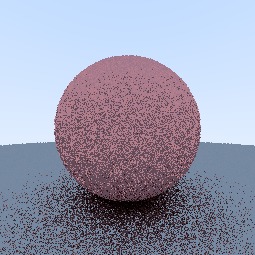
\includegraphics[width=\textwidth]{images/sampleCount/1.png}
        \caption{$n=1$}
        \label{fig:samples n equals 1}
    \end{subfigure}
    \begin{subfigure}[b]{0.2\textwidth}
        \centering
        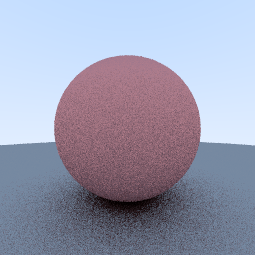
\includegraphics[width=\textwidth]{images/sampleCount/10.png}
        \caption{$n=10$}
        \label{fig:samples n equals 10}
    \end{subfigure}
    \begin{subfigure}[b]{0.2\textwidth}
        \centering
        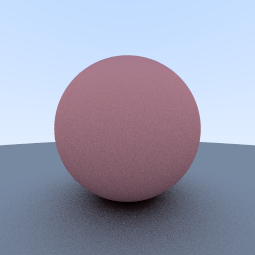
\includegraphics[width=\textwidth]{images/sampleCount/100.png}
        \caption{$n=100$}
        \label{fig:samples n equals 100}
    \end{subfigure}
    \begin{subfigure}[b]{0.2\textwidth}
        \centering
        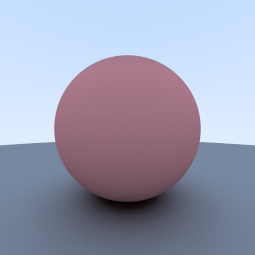
\includegraphics[width=\textwidth]{images/sampleCount/1000.png}
        \caption{$n=1000$}
        \label{fig:samples n equals 1000}
    \end{subfigure}
\end{figure}

The next parameter of interest is the maximum depth of recursion. As \cref{fig:recursion}
demonstrates, if a maximum depth of one is used, only light emitting objects are drawn, as no
reflections are computed. As the recursion depth increases, then the number of reflections also
increases. While the appearance of deeper reflections in metallic surfaces is the obvious outcome,
an additional outcome is more accurate shadows. As can be seen in \cref{fig:recursion d equals 60},
the shadows underneath the  two spheres become much lighter, and the ground under the yellow sphere
has the expected yellow tint to it.

\begin{figure}
    \caption{ The effect of recursion depth on image quality. This is an image of two metallic
        spheres, immediately in front and behind the camera, rendered with $d$ max recursion depth.
        Note that, because the camera has no ray collision logic, it remains invisible.}
    \label{fig:recursion}
    \centering
    \begin{subfigure}[b]{0.2\textwidth}
        \centering
        
\includegraphics[width=\textwidth]{images/recursiveDepth/1.png}
        \caption{$d=1$}
        \label{fig:recursion d equals 1}
    \end{subfigure}
    \begin{subfigure}[b]{0.2\textwidth}
        \centering
        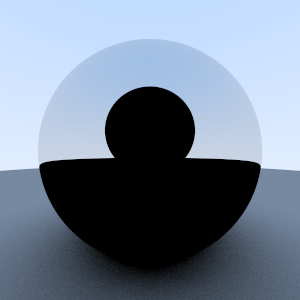
\includegraphics[width=\textwidth]{images/recursiveDepth/2.png}
        \caption{$d=2$}
        \label{fig:recursion d equals 2}
    \end{subfigure}
    \begin{subfigure}[b]{0.2\textwidth}
        \centering
        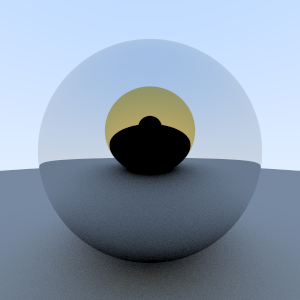
\includegraphics[width=\textwidth]{images/recursiveDepth/3.png}
        \caption{$d=3$}
        \label{fig:recursion d equals 3}
    \end{subfigure}
    \begin{subfigure}[b]{0.2\textwidth}
        \centering
        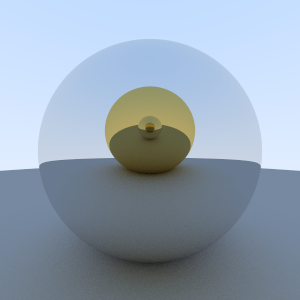
\includegraphics[width=\textwidth]{images/recursiveDepth/60.png}
        \caption{$d=60$}
        \label{fig:recursion d equals 60}
    \end{subfigure}
\end{figure}

The last parameter to discuss is the roughness parameter of a metallic material. The image in
\cref{fig:roughness} shows the transition from completely smooth to completely rough. It can also be
seen that a fully rough metal material is still behaves differently than a lambertian type material.
This difference is caused by rough metals' still maintaining directionality, while the lambertian
materials scattering is completely random.

\begin{figure}

    \caption{ Four metallic spheres with roughness values (from left to right) of 0, $1/3$, $2/3$,
        and 1, as well as a lambertial sphere for comparison.}

    \label{fig:roughness}
    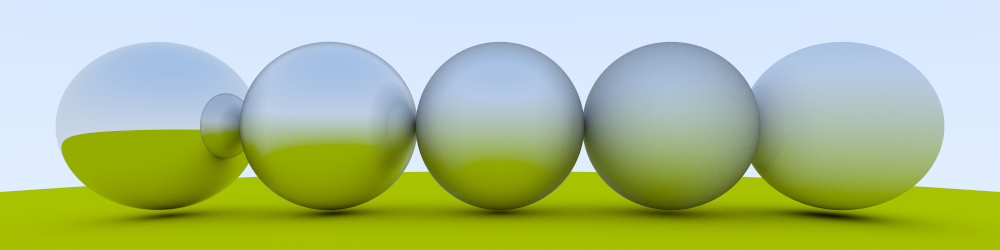
\includegraphics[width=\columnwidth]{images/roughness.png}
\end{figure}

\section*{Conclusion}

Ray-tracing based rendering algorithms while extremely computationally expensive, produce strikingly
realistic imagery. By using stochastic methods to simulate light as it behaves in real photography,
details that would take meticulous care and on the part of an artist to replicate are generated for
automatically by the algorithm. This detail comes with the cost of incredibly long run times, but
the results have justified those costs for every field where it is feasible to use.

\printbibliography

% \end{multicols*}
\end{document}
